\documentclass[runningheads]{llncs}

\usepackage[T1]{fontenc}
\usepackage{graphicx}
\usepackage{amsmath}
\usepackage{booktabs}
\usepackage{hyperref}
\usepackage{multirow}
\usepackage{placeins}
\usepackage[margin=2.2cm]{geometry}
\usepackage[skip=3pt]{caption}
\setlength{\intextsep}{4pt}
\setlength{\textfloatsep}{6pt}
\setlength{\abovecaptionskip}{2pt}

\graphicspath{{../results/figures/}}

\begin{document}

\title{Tabular and Semi-Gradient RL on Text Flappy Bird}
\author{Daniel Fernández de la Mela}
\institute{CentraleSupélec, Université Paris-Saclay \\
\email{daniel.fernandezdelamela@student-cs.fr}}
\maketitle

%─────────────────────────────────────────────────────────────────────
\section{Experimental Setup (Q1)}

We implement and compare two agents on \texttt{TextFlappyBird-v0}
(observations: integer $(\Delta x, \Delta y)$ distances to the next pipe gap;
actions: $\{0\text{=no-flap},\,1\text{=flap}\}$; reward: $+1$ per step survived).

\textbf{Agent 1 — Constant-$\alpha$ First-Visit MC Control.}
Generates complete episodes under $\varepsilon$-greedy exploration, then updates
the Q-table for each first-visited $(s,a)$ pair using the discounted return $G_t$:
\begin{equation}
  Q(s,a) \leftarrow Q(s,a) + \alpha\bigl(G_t - Q(s,a)\bigr)
\end{equation}
States are integer tuples used as direct hash keys (no discretization needed).

\textbf{Agent 2 — True Online Sarsa($\lambda$) \cite{sutton2018}.}
Updates weights at every step via linear approximation
$\hat{q}(s,a,\mathbf{w})=\mathbf{w}^\top\mathbf{x}(s,a)$
with Dutch eligibility traces (S\&B §12.7):
\begin{gather}
  \delta = R + \gamma\hat{q}(S',A',\mathbf{w}) - \hat{q}(S,A,\mathbf{w}) \\
  \mathbf{z} \leftarrow \gamma\lambda\mathbf{z} + (1-\alpha\gamma\lambda\,\mathbf{z}^\top\mathbf{x})\,\mathbf{x} \\
  \mathbf{w} \leftarrow \mathbf{w} + \alpha(\delta+q-q_\text{old})\mathbf{z} - \alpha(q-q_\text{old})\mathbf{x}
\end{gather}
Features $\mathbf{x}(s,a)$ use tile coding: 8 tilings $\times$ $8{\times}8$ tiles,
IHT size 4096, $\alpha=\alpha_\text{base}/8$.

\textbf{Key differences.} Both agents are trained for 50\,000 episodes per seed
(3 seeds), with $\varepsilon$ decaying from 1.0 to 0.05 at rate 0.9999 per episode.
Training convergence and eval curves are shown in Fig.~\ref{fig:curves}.

\begin{figure}[!ht]
  \centering
  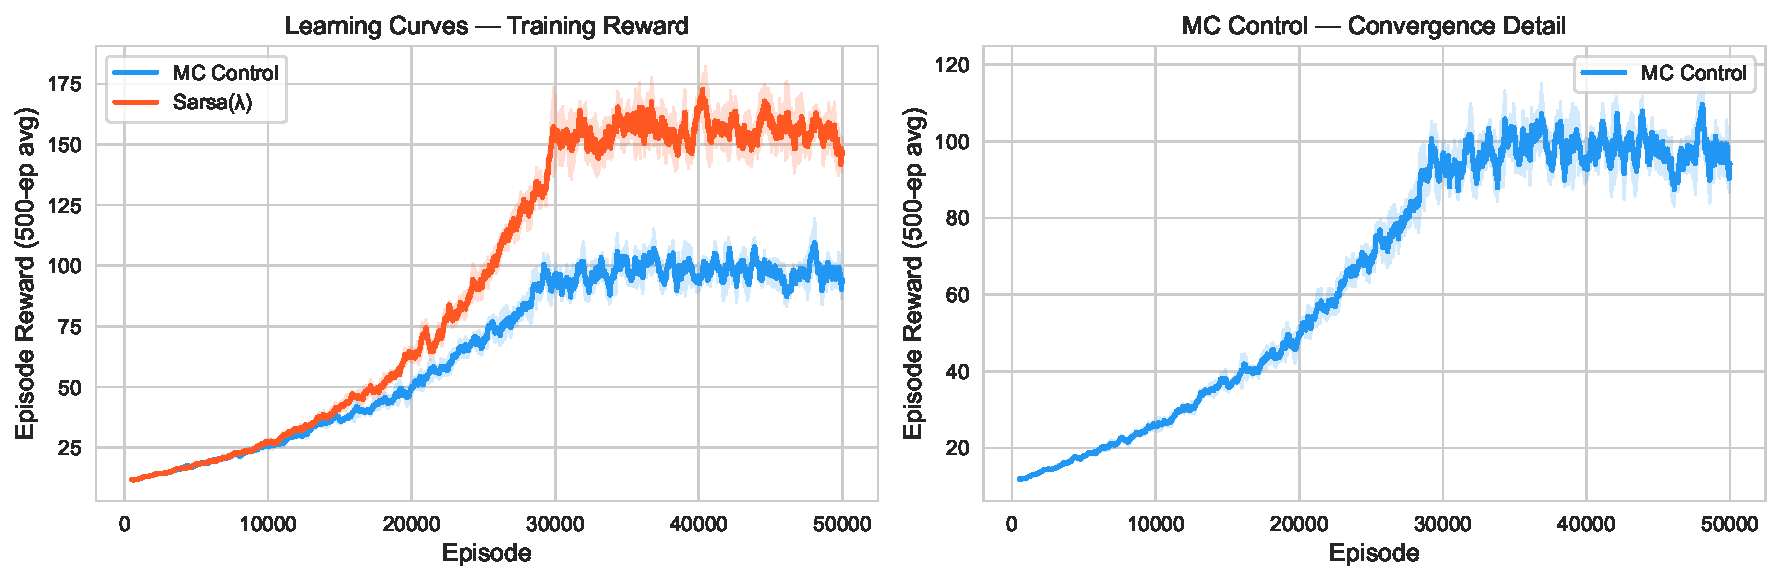
\includegraphics[width=0.88\linewidth]{fig1_learning_curves.pdf}
  \caption{Learning curves (mean $\pm$ std, 3 seeds, 500-ep smoothing). Left: both agents. Right: MC detail.}
  \label{fig:curves}
\end{figure}

MC Control trains in $\approx$60\,s/seed (274-state Q-table); Sarsa($\lambda$)
requires $\approx$500\,s/seed ($8\times$ slower, 978/4096 non-zero weights).
Both plateau around episode 30\,000.
Under default hyperparameters (MC: $\alpha=0.1$, $\gamma=0.99$; Sarsa: $\alpha_\text{base}=0.2$, $\lambda=0.9$),
eval scores over 50 greedy episodes are:
MC seeds 0–2: $206\pm223$, $400\pm259$, $170\pm164$;
Sarsa seeds 0–2: $1950\pm1909$, $603\pm567$, $370\pm336$.
Sarsa achieves higher but more variable performance — a bimodal distribution
typical of Flappy Bird where one suboptimal decision cascades into immediate death.

%─────────────────────────────────────────────────────────────────────
\section{State/Action-Value Functions}

Figure~\ref{fig:values} shows the learned value function $V(s)=\max_a Q(s,a)$
and greedy policy $\pi(s)$ for both agents after training.

\begin{figure}[!ht]
  \centering
  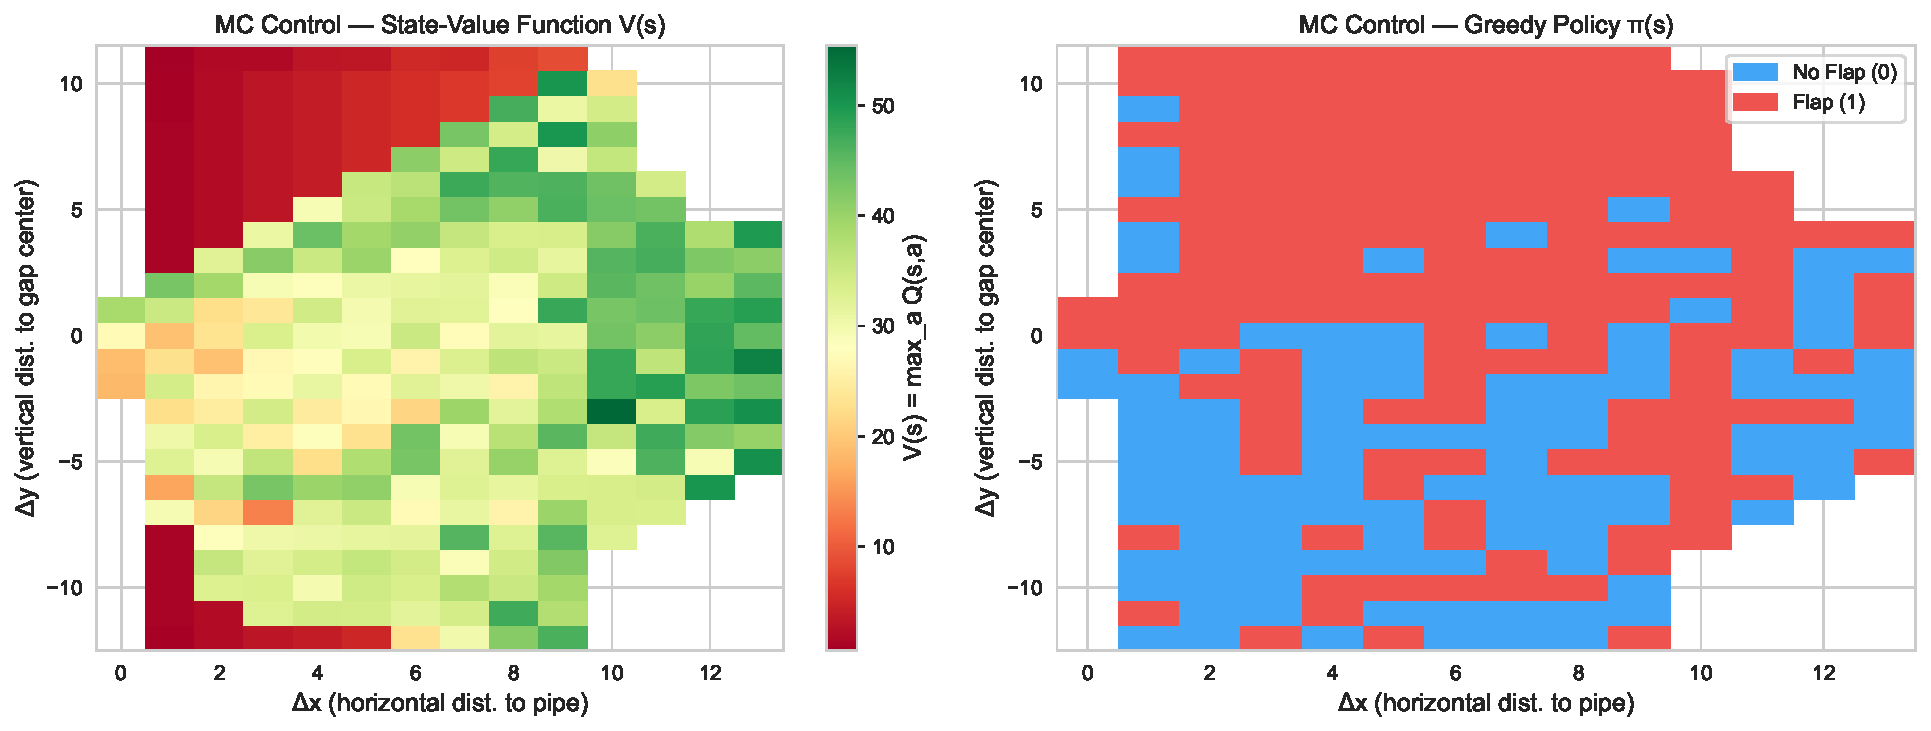
\includegraphics[width=0.72\linewidth]{fig2_mc_value_policy.pdf}\\[2pt]
  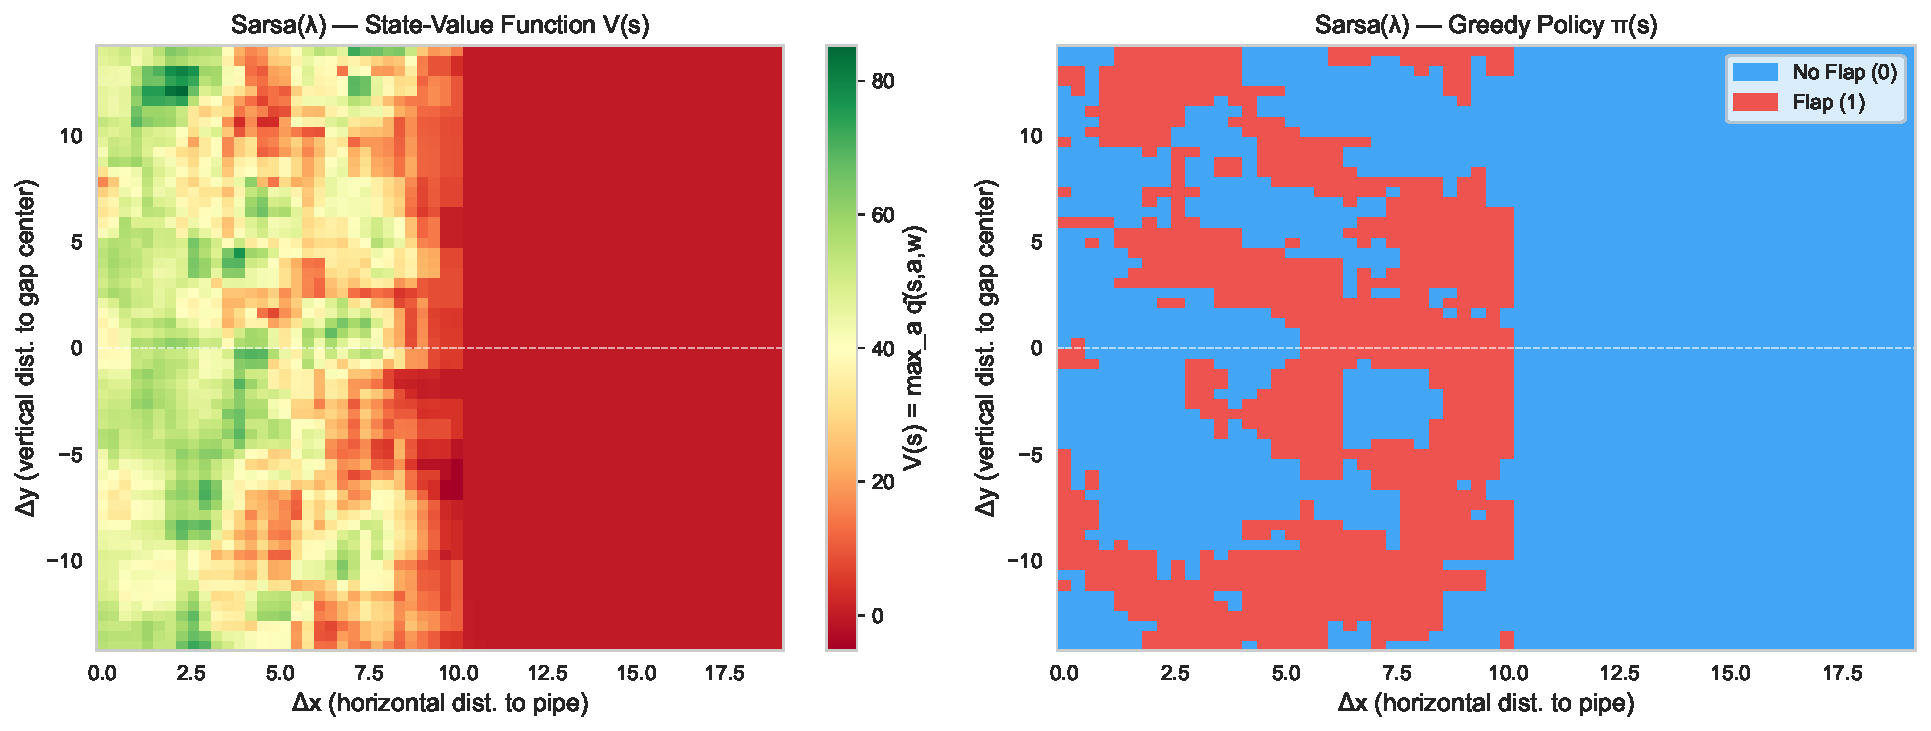
\includegraphics[width=0.72\linewidth]{fig3_sarsa_value_policy.pdf}
  \caption{Value function V(s) and greedy policy. Top: MC (Q-table, 274 states). Bottom: Sarsa($\lambda$) (weight vector). Blue=No Flap, Red=Flap; dashed=$\Delta y{=}0$.}
  \label{fig:values}
\end{figure}

Both agents (Fig.~\ref{fig:values}) learn the correct policy: flap below the gap ($\Delta y<0$), do nothing above.
MC's map covers only the 274 visited integer states — coarse but exact.
Sarsa's is smooth: tile coding generalizes across unvisited states, visible in the gradient structure
absent from MC. Values peak near $\Delta y=0$ (gap center) and drop towards boundaries.

%─────────────────────────────────────────────────────────────────────
\section{Parameter Sweeps (Q1 cont.)}

\begin{figure}[!ht]
  \centering
  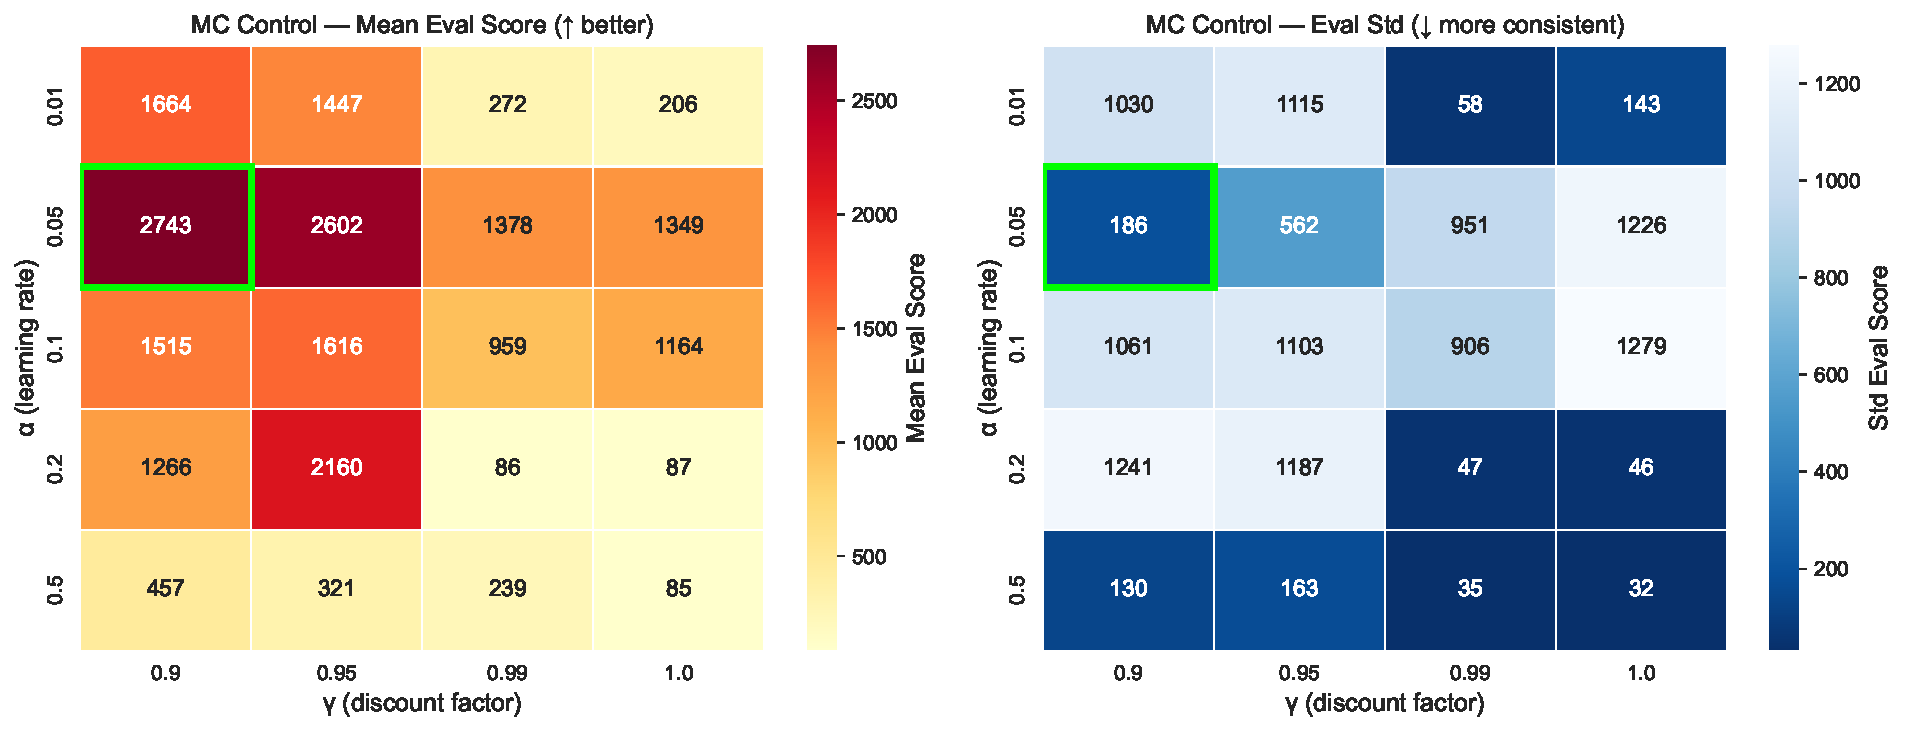
\includegraphics[width=0.84\linewidth]{fig4_sweep_mc.pdf}\\[2pt]
  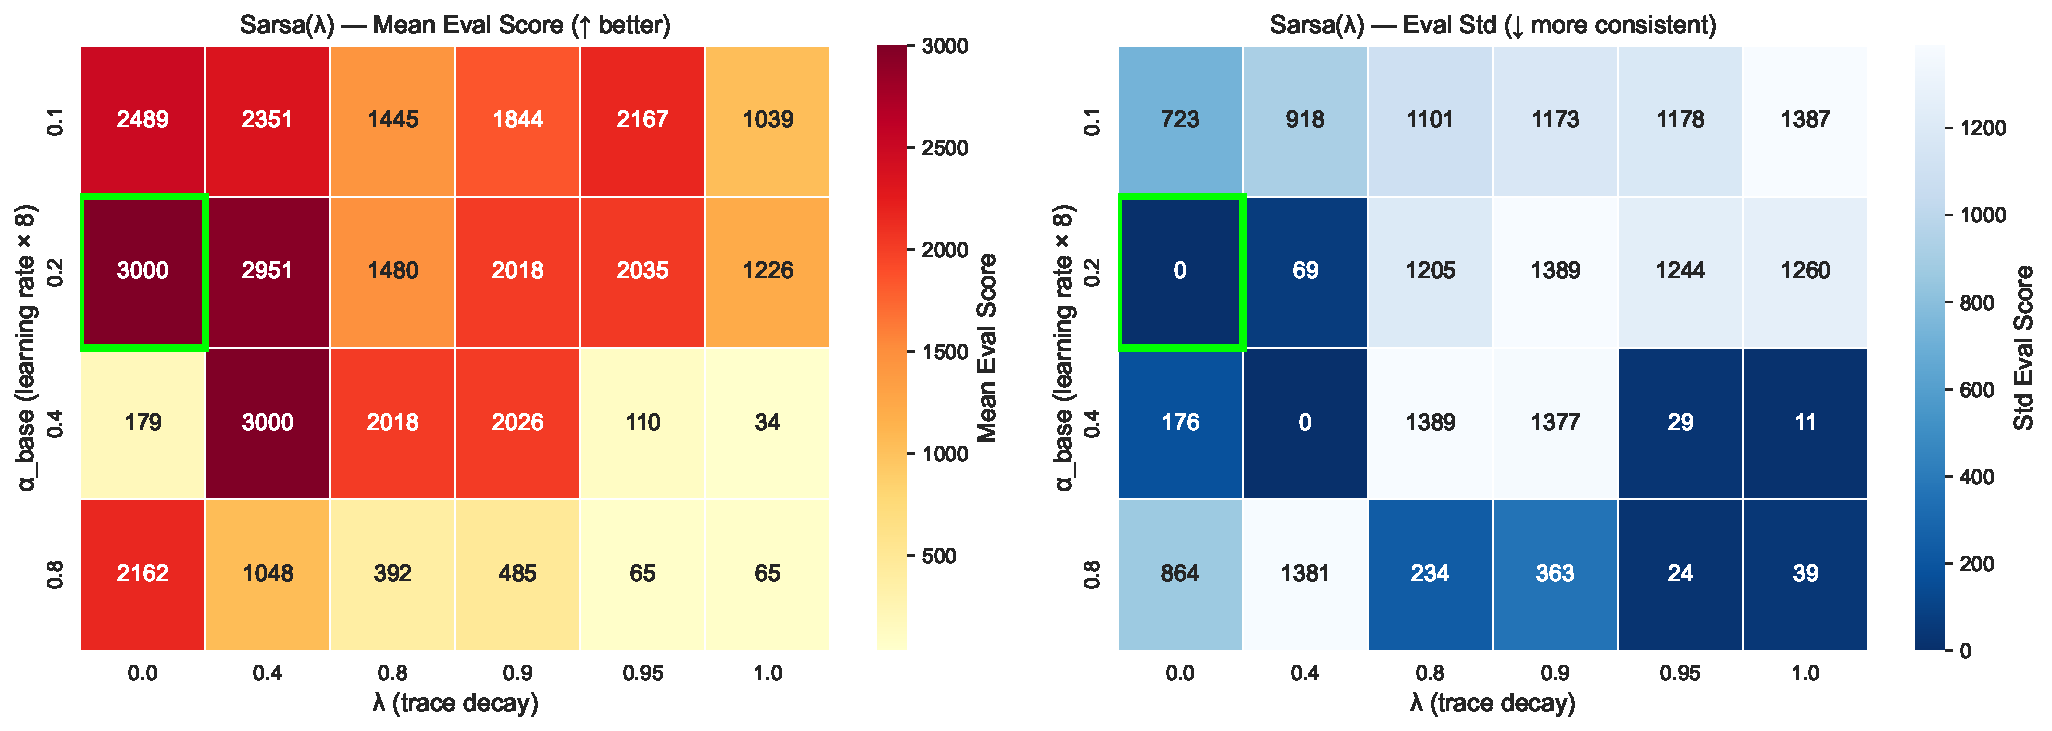
\includegraphics[width=0.84\linewidth]{fig5_sweep_sarsa.pdf}
  \caption{Parameter sweeps (3 seeds, 30\,000 ep.). \textbf{Top}: MC Control ($\alpha\times\gamma$); green = best ($\alpha=0.05$, $\gamma=0.9$, mean 2743). \textbf{Bottom}: Sarsa($\lambda$) ($\alpha_\text{base}\times\lambda$); green = best; 3000 = eval cap (perfect).}
  \label{fig:sweeps}
\end{figure}

\textbf{MC Control} (Fig.~\ref{fig:sweeps}, top):
Best config $\alpha=0.05$, $\gamma=0.9$ (mean eval 2743, std 186).
$\gamma=0.9$ outperforms $\gamma=0.99$: the effective horizon $1/(1-\gamma)\approx10$
steps matches the decision scale of TFB (one pipe). Higher $\gamma$ over-weights
distant, hard-to-control events.

\textbf{Sarsa($\lambda$)} (Fig.~\ref{fig:sweeps}, bottom):
Two configs reach the cap (3000/3000 with zero variance): ($\alpha_\text{base}=0.2$, $\lambda=0.0$)
and ($\alpha_\text{base}=0.4$, $\lambda=0.4$). Configs with $\lambda\geq0.95$ collapse:
long traces propagate credit beyond the 1–2 step consequence window of each flap.
$\lambda=0$ (TD(0)) is optimal — credit assignment is exact for this short-horizon task.

%─────────────────────────────────────────────────────────────────────
\section{Additional Experiments}

\subsection{TFB-v0 vs screen-v0 (Q2)}

\texttt{TextFlappyBird-v0} exposes $(\Delta x,\Delta y)$ — a minimal sufficient
statistic — enabling tabular MC with only 274 states.
\texttt{TextFlappyBird-screen-v0} provides the full rendered frame (hashed to
tuples for MC): the Q-table grows to 10\,075 states ($37\times$ larger), yet MC
scores 1815$\,\pm\,$1051, below the cap. The screen encodes irrelevant layout
features (pipe walls, borders) that inflate the state space without adding
decision-relevant information. Sarsa($\lambda$) tile coding is inapplicable to
screen observations without a compact embedding.

\subsection{Original Flappy Bird (Q3)}

\texttt{flappy-bird-gym} \cite{flappybird} returns RGB frames
($512\!\times\!288\!\times\!3$). MC is impractical (state space never repeats);
Sarsa tile coding assumes low-dimensional inputs. Both agents \emph{could} work
given a hand-crafted feature extractor (e.g., extracting pipe distances from pixels),
but are inapplicable out-of-the-box. Deep RL (DQN, PPO) is the appropriate choice
for raw pixel environments.

\subsection{Generalization to Different Configurations (Q4)}

\begin{table}[!ht]
\centering
\caption{Generalization: trained on default (H=15, W=20, g=4), tested zero-shot (seed 42, 100 ep.).}
\label{tab:gen}
\begin{tabular}{lcc}
\toprule
Configuration & MC eval & Sarsa eval \\
\midrule
Baseline ($g=4$, same)    & $240\pm205$ & $202\pm200$ \\
Harder ($g=3$)            & $21\pm18$   & $22\pm14$   \\
Easier ($g=6$)            & $747\pm686$ & $645\pm589$ \\
Bigger screen (20×30)     & $4\pm0$     & $4\pm0$     \\
Smaller screen (10×15)    & $105\pm104$ & $62\pm63$   \\
\bottomrule
\end{tabular}
\end{table}

Results (Table~\ref{tab:gen}) show performance scales with gap size but fails completely
on unseen screen sizes. The 20$\times$30 grid scores $4\pm0$ for both — immediate death:
MC has no Q-values for the new integer states; Sarsa's tile boundaries map to
out-of-distribution features. The smaller screen partially transfers for MC (105) but
less for Sarsa (62). Both agents learn environment-specific rather than geometry-invariant policies.

\FloatBarrier
%─────────────────────────────────────────────────────────────────────
\begin{thebibliography}{3}
\bibitem{sutton2018}
Sutton, R.S., Barto, A.G.: Reinforcement Learning: An Introduction, 2nd edn. MIT Press (2018)
\bibitem{tfb}
Christodoulidis, S.: Text Flappy Bird Gym.
\url{https://gitlab-research.centralesupelec.fr/stergios.christodoulidis/text-flappy-bird-gym} (2022)
\bibitem{flappybird}
Talendar: Flappy Bird Gym.
\url{https://github.com/Talendar/flappy-bird-gym} (2021)
\end{thebibliography}

\end{document}
